\PassOptionsToPackage{x11names}{xcolor}
\documentclass[3to2]{beamer}

\beamertemplatenavigationsymbolsempty

\usepackage{mathpartir}
\usepackage{bytefield}
\usepackage{tcolorbox}
\usetheme{jambro}
\usetikzlibrary{shapes}
\usepackage{catchfilebetweentags}
\makeatletter

\newrobustcmd*\OrigExecuteMetaData[2][\jobname]{%
\CatchFileBetweenTags\CatchFBT@tok{#1}{#2}%
\global\expandafter\CatchFBT@tok\expandafter{%
\expandafter}\the\CatchFBT@tok
}%\OrigExecuteMetaData

\newrobustcmd*\ChkExecuteMetaData[2][\jobname]{%
\CatchFileBetweenTags\CatchFBT@tok{#1}{#2}%
\edef\mytokens{\detokenize\expandafter{\the\CatchFBT@tok}}
\ifx\mytokens\empty\PackageError{catchfilebetweentags}{the tag #2 is not found\MessageBreak in file #1 \MessageBreak called from \jobname.tex}{use a different tag}\fi%
}%\ChkExecuteMetaData

\renewrobustcmd*\ExecuteMetaData[2][\jobname]{%
\ChkExecuteMetaData[#1]{#2}%
\OrigExecuteMetaData[#1]{#2}%
}

\makeatother

\usepackage{idris2}
\usepackage{transparent}
\usepackage{multirow}

\newcommand{\cowhead}{
\includegraphics[scale=.17]{assets/TYPES-cow.png}}
\newcommand{\mastodon}{
\includegraphics[scale=.2]{assets/mastodon-logo-purple.png}}
\newcommand{\globe}{
\includegraphics[scale=.1]{assets/globe.png}}


\newcommand<>\hlon[1]{\alt#2{\colorbox{carandache}{#1}}{#1}}

\newcommand{\nat}{\ensuremath{\mathbb{N}}}
\newcommand{\str}{\ensuremath{\mathbb{S}}}
\newcommand{\recvar}[1]{\ensuremath{\mathit{#1}}}
\newcommand{\send}[2]{\ensuremath{!#1.\;#2}}
\newcommand{\recv}[2]{\ensuremath{?#1.\;#2}}
\newcommand{\select}[2]{\ensuremath{#1 \mathop{\oplus} #2}}
\newcommand{\offer}[2]{\ensuremath{#1 \mathop{\&} #2}}
\newcommand{\smallest}[2]{\ensuremath{\mu #1.\;#2}}
\newcommand{\largest}[2]{\ensuremath{\nu #1.\;#2}}
\newcommand{\stopsesh}{\ensuremath{\mathtt{end}}}

\usepackage{tikz}
\usetikzlibrary{automata, positioning, arrows}
\tikzset{
  ->, % makes the edges directed
  >=stealth', % makes the arrow heads bold
  node distance=3cm, % specifies the minimum distance between two nodes. Change if necessary.
  every state/.style={thick, fill=gray!10, minimum size=1cm}, % sets the properties for each ’state’ node
  initial text=$ $, % sets the text that appears on the start arrow
}


\tikzset{
    invisible/.style={opacity=0,text opacity=0},
    visible on/.style={alt=#1{}{invisible}},
    alt/.code args={<#1>#2#3}{%
      \alt<#1>{\pgfkeysalso{#2}}{\pgfkeysalso{#3}}
    },
}
\tikzset{
  background fill/.style={fill=#1},
  background fill/.default={gray!10},
  fill on/.style={alt=#1{}{background fill}},
}



\title{Type-safe Bidirectional Channels in Idris 2}
\author{Guillaume Allais}
\institute{University of Strathclyde \\ Glasgow, UK}
  \titlegraphic{TYPES}
\date{June 12$^{th}$ 2025}

\setbeamertemplate{section in toc}{\inserttocsection}
\AtBeginSection[]
{
    \begin{frame}
        \frametitle{Table of Contents}
        \tableofcontents[currentsection]
    \end{frame}
}

\usepackage{listings}
\lstset{language=Fortran,
  basicstyle=\ttfamily\bf,
  keywordstyle=\color{red},
}

%% Disable the >> ligature
\usepackage{microtype}
\DisableLigatures[>]{}

\begin{document}

\begin{frame}
  \maketitle
\begin{tikzpicture}[remember picture, overlay]
  \node[anchor=south east] at ($(current page.south east)+(0,.27)$){\cowhead};
\end{tikzpicture}
\end{frame}

\begin{frame}{Table of Contents}
  \tableofcontents
\end{frame}

\begin{frame}{Session types}
  \begin{align*}%
  p,~ q,~ \dots &
    \; ::= \; \recvar{x}
    \; | \; \smallest{x}{p}
    \; | \; \largest{x}{p} \\
    &
    \; | \; \send{A}{p}
    \; | \; \recv{A}{p}
    \; | \; \stopsesh{} \\
    &
    \; | \; \offer{p}{q}
    \; | \; \select{p}{q}
  \end{align*}
\end{frame}

\begin{frame}{The ``adder'' server protocol}

$$
\largest{\hlon<6>{\recvar{i}}}{\hlon<2>{(\offer
  {\hlon<3>{(\send{\nat}{\hlon<4>{\stopsesh}})}}
  {\hlon<5>{(\recv{\nat}{\hlon<6>{\recvar{i}}})}})}}
$$
\begin{center}
  \begin{tikzpicture}
    \node[state, initial, fill=carandache, fill on=<{2,6}>] (q1) {init};
    \node[state, below of=q1, fill=carandache, fill on=<3>] (q2r) {eval};
    \node[state, right of=q1, fill=carandache, fill on=<5-6>]                (q2l) {more};
    \node[state, accepting, right of=q2r, fill=carandache, fill on=<4>]     (q3)  {stop};

    \draw<1-5> (q1) edge[bend left, above]  node{false}       (q2l);
    \draw<6>  (q1) edge[bend left, above, pencil]  node{false}       (q2l);
    \draw<1-5> (q2l) edge[bend left, below] node{recv \nat} (q1);
    \draw<6>   (q2l) edge[bend left, below, pencil] node{recv \nat} (q1);
    \draw  (q1) edge[left]      node{true}       (q2r)
      (q2r) edge[above]            node{send \nat} (q3);
  \end{tikzpicture}
\end{center}

\end{frame}

\begin{frame}

  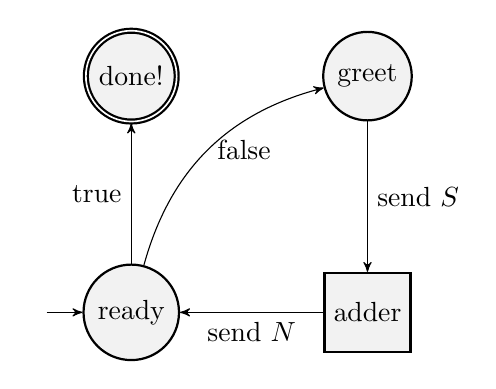
\begin{tikzpicture}
    \node[state, initial]                      (o1)  {ready};
    \node[state, above of=o1, accepting] (o2)  {done!};
    \node[state, right of=o2] (o3)  {greet};
    \node[state, shape=rectangle, below of=o3] (q1)  {adder};
    \draw
      (o1) edge[bend left, right] node{false} (o3)
      (o1) edge[left]            node{true}  (o2)
      (o3) edge[right] node{send \str} (q1)
      (q1) edge[below] node{send \nat} (o1);
  \end{tikzpicture}
\end{frame}

\begin{frame}
$$
\largest{\hlon<7>{\recvar{r}}}{\hlon<2>{(\offer{\hlon<3>{\stopsesh}}
  {\hlon<4>{(\send{\str}{\hlon<5>{\largest{\hlon<6>{\recvar{i}}}{(\offer
  {(\send{\nat}{\hlon<7>{\recvar{r}}})}}
  {(\recv{\nat}{\hlon<6>{\recvar{i}}}))}}
  )}})}}}
$$
\begin{center}
  \begin{tikzpicture}
    \node[state, initial, fill=carandache, fill on=<{2,7}>] (o1)  {ready};
    \node[state, above of=o1, fill=carandache, fill on=<3>, accepting] (o2)  {done!};
    \node[state, right of=o2, fill=carandache, fill on=<{4,7}>] (o3)  {greet};
    \node[state, below of=o3, fill=carandache, fill on=<{5,6,7}>] (q1) {init};
    \node[state, below of=q1, fill=carandache, fill on=<{5,7}>] (q2r) {eval};
    \node[state, right of=q1, fill=carandache, fill on=<{5,6,7}>] (q2l) {more};

    \draw
      (o1) edge[left]            node{true}  (o2);
    \draw<1-6>
      (o1) edge[bend left, right] node{false} (o3)
      (o3) edge[right] node{send \str} (q1)
      (q2r) edge[bend left, left] node{send \nat} (o1)
      (q1) edge[left]      node{true}       (q2r);
    \draw<1-5> (q1) edge[bend left, above]  node{false}       (q2l);
    \draw<6-7>  (q1) edge[bend left, above, pencil]  node{false}       (q2l);
    \draw<1-5> (q2l) edge[bend left, below] node{recv \nat} (q1);
    \draw<6-7>   (q2l) edge[bend left, below, pencil] node{recv \nat} (q1);
    \draw<7>
      (o1) edge[bend left, right, pencil] node{false} (o3)
      (o3) edge[right, pencil] node{send \str} (q1)
      (q2r) edge[bend left, left, pencil] node{send \nat} (o1)
      (q1) edge[left, pencil]      node{true}       (q2r);
  \end{tikzpicture}
\end{center}
\end{frame}

\begin{frame}{Our End Goal}
\noindent\begin{minipage}[t]{.49\textwidth}
  \ExecuteMetaData[System/Concurrency/Session/MuNuN.idr.tex]{server}
\end{minipage}
\begin{minipage}[t]{.49\textwidth}
  \ExecuteMetaData[System/Concurrency/Session/MuNuN.idr.tex]{adder}
\end{minipage}
\end{frame}


\begin{frame}{What's next?}
\end{frame}

\end{document}
